\section{The Landscape of Rationality for Relations over Finite Words}
\label{sec:preliminaries-automatic-structures-relations}

\subsection{Regularity is Key}
\label{sec:preliminaries-automatic-structures-relations-landscape}

The study of classes of relations on words have always been a central topic in language theory
\cite{ElgotMezi1965RelationsGeneralizedAutomata,Nivat1968TransductionChomsky,Berstel1979Transductions,FrougnySakarovitch1993SynchronizedRationalRelations,Choffrut2006Survey}. 
More recently, their study has also been motivated by database theory and verification,
where they are used to build expressive languages. For instance,
suitable classes of word relations where shown to be relevant for querying strings over relational 
databases \cite{BenediktLibkinSchwentickSegoufin2003DefinableRelations}, comparing paths in graph databases \cite{BarceloLibkinLinWood2012ExpressiveLanguages}---see also \cite[\S 8, p.~17]{Figueira2021FoundationsGraphPathQueryLanguages}
for more context \& results on \emph{extended} conjunctive regular path queries---, or defining string constraints for model checking \cite{LinBarcelo2016StringSolvingWordEquationsTransducers}. 
% The most studied such classes include "recognizable@@rel", "automatic@@rel" "aka" "synchronous@@rel", and "rational relations", each one of the latter two strictly extending the previous one. 
We start by showing that, while the notion of "regular language" is canonical and admits 
numerous characterizations, these definitions are no longer equivalent when dealing
with finite word relations, leading to a \emph{hierarchy} of notions of \emph{rationality}.

The class of "regular languages" is remarkably stable, and can be characterized as the 
languages recognized by either:
\begin{itemize}
	\item deterministic or non-deterministic finite state automata,\\
		\null\hspace{1.0pc}see "eg" \cite[Proposition~1.2.3, p.~7]{Pin2021FiniteAutomata};
	\item two-way finite state automata by Shepherdson-Rabin-Scott theorem\\
		\null\hspace{1.0pc}\cite[Theorem~2, p.~198]{Shepherdson1959ReductionTwoWay}
		\cite[Theorem~15, p.~123]{RabinScott1959FiniteAutomata};
	\item rational expressions\footnote{Usually called ``regular expressions'' by
		non-French speakers, however we use the terminology ``rational'' for its unambiguity.}
		by Kleene's theorem,\\
		\null\hspace{1.0pc}see "eg" \cite[Theorem~1.5.11, p.~34]{Pin2021FiniteAutomata};
	\item monadic second-order logic by Trakhtenbrot-Büchi-Elgot theorem,\\
		\null\hspace{1.0pc}see "eg" \cite[Theorem~2.2, p.~32]{Bojanczyk2020MSO}; or
	\item finite monoids, see "eg" \cite[\S~1.4.2, p.~19]{Pin2021FiniteAutomata}.
\end{itemize}
Moreover, all transformations between these representations are effective---although some
models are strictly more succinct than others.

\begin{figure*}
	\centering
	\begin{tikzpicture}
		\tikzset{
			ex/.style={
				font={\small\sffamily},
			},
			class/.style={
				align=center,
				font={\footnotesize\scshape\sffamily},
			}
		}

		\node at (0,0) {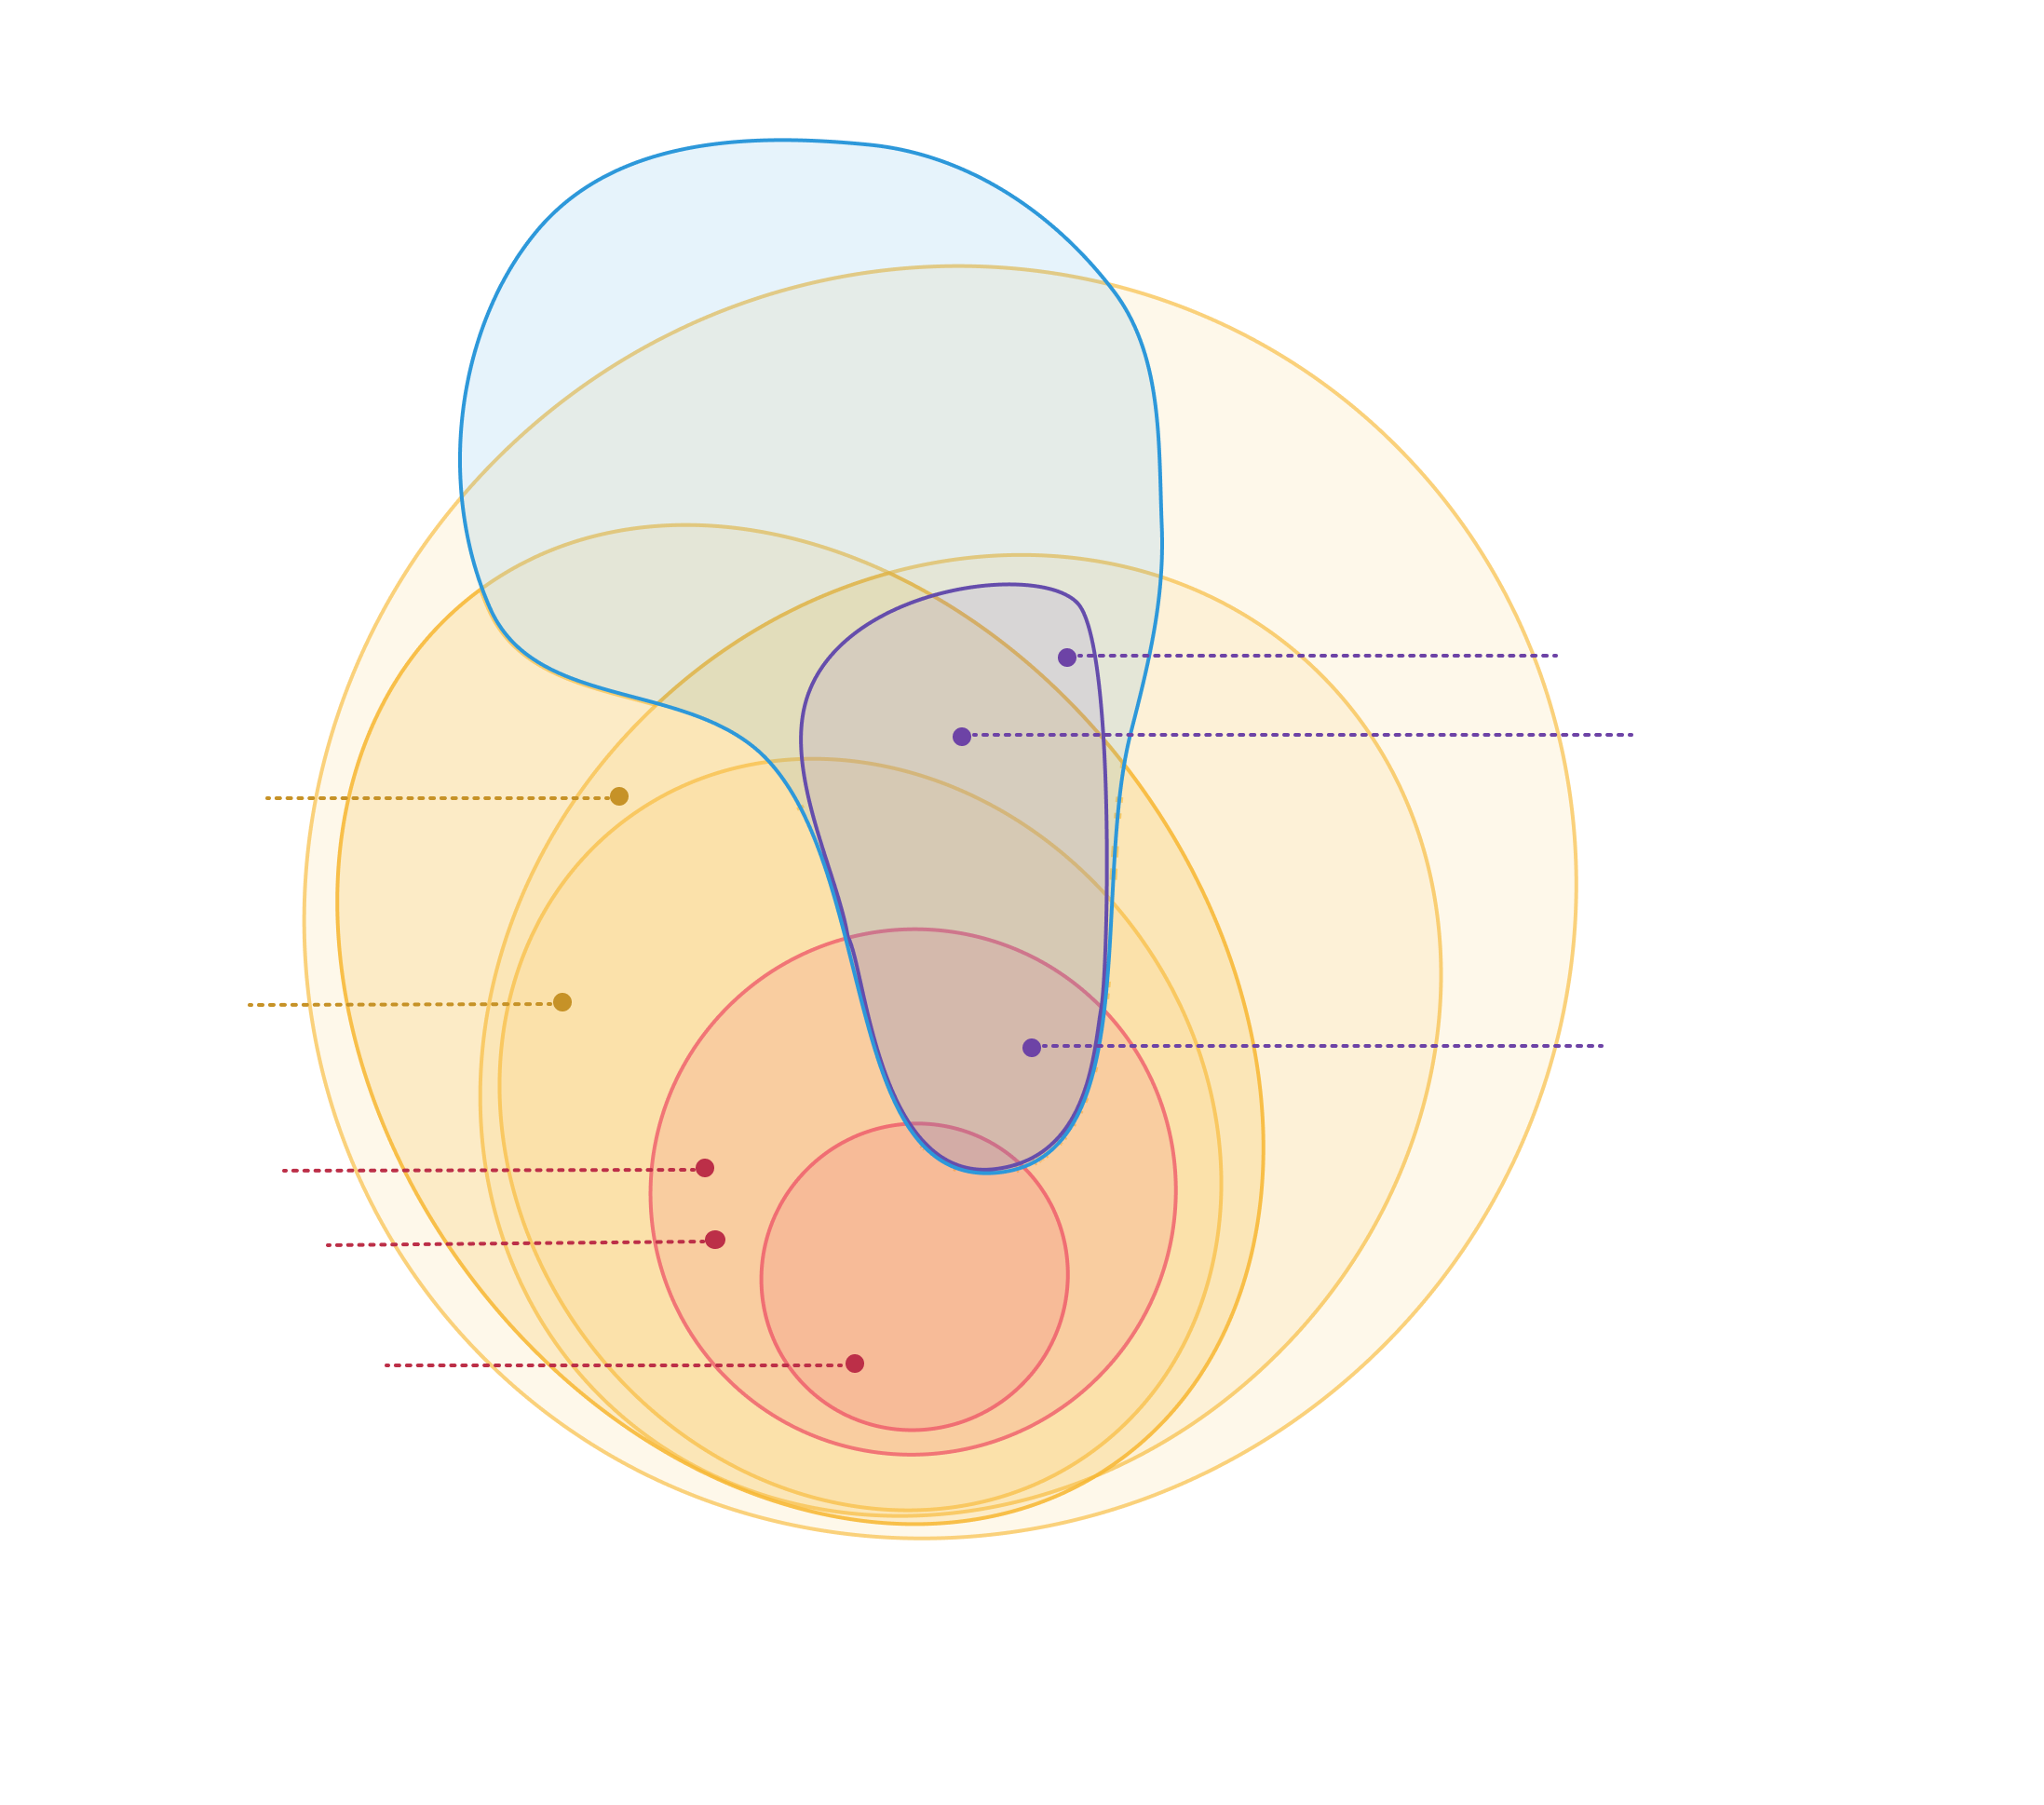
\includegraphics[width=.9\linewidth]{fig/prelim-automatic/landscape-rationality-relations.png}};
		% \draw[step=0.2,cGrey,thin] (-8,-5) grid (8,6);
		% \draw[step=1,black,thin] (-8,-5) grid (8,6);
		% \draw[black, thick] (-8, 0) to (8,0);
		% \draw[black, thick] (0,-5) to (0,6);

		\node[ex, left] at (-5,-3.55)
			{\kl[same parity length relation]{\textcolor{cRed!80!black}{same parity length relation}}};
		\node[ex, left] at (-5.5,-2.65)
			{\kl[\equalLength]{\textcolor{cRed!80!black}{equal length relation}}};
		\node[ex, left] at (-5.8,-2.05)
			{\kl[prefix relation]{\textcolor{cRed!80!black}{prefix relation}}};
		\node[ex, right] at (4.5,-1.1)
			{\kl[identity relation]{\textcolor{cPurple!80!black}{identity function}}};
		\node[ex, right, align=left, text width=3.5cm] at (4.7,1.1)
			{\textcolor{cPurple!80!black}{`greatest suffix in $L$'\\[-.2em] function}};
		\node[ex, right] at (4.2,1.9)
			{\textcolor{cPurple!80!black}{palindrome function}};
		\node[ex, left] at (-6,-0.8)
			{\kl[subword relation]{\textcolor{cYellow!80!black}{subword relation}}};
		\node[ex, left] at (-5.8,0.8)
			{\kl[suffix relation]{\textcolor{cYellow!80!black}{suffix relation}}};

		\node[class, text width=1.8cm] at (-0.8,-2.8)
			{\kl[recognizable relations]{\textcolor{cRed!80!black}{Recognizable relations}}};
		\node[class, text width=1.8cm] at (-1.85,-1.4)
			{\kl[automatic relations]{\textcolor{cRed!80!black}{Automatic relations}}};
		\node[class, text width=2.1cm] at (-2.5,-.12)
			{\kl[deterministic rational relations]{\textcolor{cYellow!80!black}{Det\ic\ rational relations}}};
		\node[class, text width=1.5cm] at (-4.1,1.3)
			{\kl[rational relations]{\textcolor{cYellow!80!black}{Rational relations}}};
		\node[class, text width=2.1cm] at (2.2,.4)
			{\kl[deterministic two-way rational relations]{\textcolor{cYellow!80!black}{Det\ic\ two-way rational relations}}};
		\node[class, text width=2.1cm] at (2.2,3)
			{\kl[two-way rational relations]{\textcolor{cYellow!80!black}{Two-way rational relations}}};
		\node[class, text width=1.8cm] at (-2.2,5.2)
			{\kl[functional relations]{\textcolor{Boyzone!80!black}{Functional relations}}};
		\node[class, text width=1.5cm] at (-.3,.4)
			{\kl[regular functions](bojan){\textcolor{cPurple!80!black}{Regular functions}}};
	\end{tikzpicture}
	\caption{
		\AP\label{fig:landscape-rationality-relations}
		Clickable landscape of rationality for binary relations.
		See also \Cref{fig:hierarchy-rational-relations,fig:hierarchy-functional-relations}.
	}
\end{figure*}
These equivalences explain why the terms \emph{recognizable language}---meaning implicitly
``recognizable by a finite-state automaton'' or ``recognizable by a finite monoid''---and
\emph{rational language}---meaning ``described by a rational expression''---are used 
interchangeably. In fact, in this thesis as well as in most of the literature,
we will use the generic term "regular language".
However, in more complex settings, for instance subsets of non-free monoids,%
\footnote{Recall that a language is nothing else but a subset of a free
(usually finitely-generated) monoid.}
the equivalence between these classes no longer holds \cite{Pin2021StackExchange}.

The landscape of rationality for $k$-ary relations of finite words ($k \geq 2$) is far more complex than for languages,\footnote{Which can be seen as unary relations of finite words.} as depicted in \Cref{fig:landscape-rationality-relations}. We will briefly present these classes,
although this thesis will mostly deal with the two most restrictive ones, namely
"recognizable@@rel" and "automatic relations".%
\footnote{It should be noted that the names
of these classes were often coined independently of one another
and the terminology should be handled with care: for instance,
``regular relations'' do \emph{not} correspond to the intersection of "regular functions@@bojan"
with "functional relations".}

We fix two alphabets $\Gamma$ and $\Sigma$. In the rest of this section, we focus
on relations $\+R \subseteq \Gamma^* \times \Sigma^*$. We will sometimes provide definitions
for relations of higher arity when the generalization is not trivial.

\paragraph*{Goal of this section.}
Beyond introducing the classes of "recognizable@@rel" and "automatic relations", the goal of
this section is also to clarify the literature. When dealing with relations, there are essentially 
two families of machines for recognizing a relation $\+R \subseteq \Gamma^* \times \Sigma^*$:
\begin{itemize}
	\item \emph{multitape automata:} this model reads a pair of words $\tup{u,v} \in \Gamma^* \times \Sigma^*$ and decides if it belongs to $\+R$;
	\item \emph{transducers:} this model reads a word $u \in \Gamma^*$ and produces a word (or no word, or multiple words) $v\in \Sigma^*$, in which case we say that $\tup{u,v} \in \+R$.  
\end{itemize}
The latter model is inherently passive while the former is more active: the output is produced,
or \emph{transduced}, from the input. However, these two families are far from being incomparable:
when non-determinism is allowed and the model is expressive enough, a transducer can always guess the output and simulate a "multitape automata". Despite this fact, the works on "multitape automata" and "transducers" rarely reference each other, and the relationship between classes
of relations defined by these two families of models is often unclear.%
\footnote{To witness this claim, I want to emphasize that I unwillingly included an erroneous 
version of \Cref{fig:landscape-rationality-relations} in \cite{Morvan2025Algebras}:
the "suffix relation" was misplaced and, more
importantly, the "regular functions@@bojan" were claimed to correspond to
the intersection of "rational relations" with "deterministic two-way rational relations".}
For instance, we will see in \Cref{sec:prelim-transductions}
that "deterministic two-way multitape automata"
and "deterministic two-way transducers" are semantically different: the distinction
between \emph{multitape automata} and \emph{transducers} is hence of capital importance.

Thus, the goal of this section is to provide an overview of these classes of relations/transductions, explain how they relate to one another, and give pointers to suitable references.
The aim of this section is not to be exhaustive, which would be a daunting task,%
\footnote{Sakarovitch's book \cite{Sakarovitch2009Elements}
dedicates its second part to ``Rationality in relations'', which spans over more than two hundred pages---one can only imagine how extensive this part could have been if the book was not
dedicated to presenting \emph{elements} of automata theory but the full theory itself!
Note in fact that the book does not even mention two-way models.
What we call here "multitape automata" are called there ``transducers''
and our "transducers" are called ``sequential transducers'' there.
We made this choice of terminology because it seems more consistent with
the literature, and we find both more natural and more intuitive.}
but rather to present a quick overview of the most common classes of relations
studied in the literature.

\paragraph*{Relations "vs" transductions.}
Often, in the literature, when the terminology ``transduction'' is used,
these relations are thought as functions from $\Gamma^*$ to $\pset{\Sigma^*}$.
These functions are equivalent\footnote{Meaning formally that these categories are isomorphic.}
to relations, "ie" subsets of~$\Gamma^* \times \Sigma^*$.
For deterministic transducers, the output is a singleton, and hence its semantics can be seen
as a \emph{partial function}---or equivalently as a "functional relation"---from $\Gamma^*$ to $\Sigma^*$.

When the terminology ``relation'' is used,
we often take $\Gamma = \Sigma$.%
\footnote{For instance this is somewhat important when
dealing with logic or defining "automatic structures"
in \Cref{sec:preliminaries-automatic-structures-automatic-structures,sec:preliminaries-automatic-structures-logic}.}
Note also that most notions defined by multitape automata
can be trivially extended to $k$-ary relations ($k \geq 3$):
we simply work here with binary relations for the sake of simplicity.
On the other hand, transducers intrinsically recognize functions $\Gamma^* \to \pset{\Sigma^*}$,
"ie" binary relations.

Given two classes of finite-word relations $\+C$ and $\+D$ "st" $\+C \supseteq \+D$,%
\footnote{Formally, for the decision problem to make sense $\+C$ and $\+D$ should rather be
classes of machines (recognizing relations),
but we abuse the terminology for the sake of readability.}
we will often want to know if this inclusion is \emph{effective}:
\decisionproblem{
	""$\+D$-membership problem for $\+C$-relations""
}{
	A $\+C$-relation $\+R$.
}{
	Does $\+R \in \+D$?
}
This problem is also called the \reintro{$\+C$/$\+D$-membership problem}.

A natural extension of this problem is the so-called separability problem,
which has received a lot of attention.
\decisionproblem{
	""$\+D$-separability problem for $\+C$-relations""
}{
	Two $\+C$-relations $\+R$ and $\+R'$.
}{
	Is there a $\+D$-relation $\+S$ "st" $\+R \subseteq \+S$ and $\+R' \cap \+S = \emptyset$?
}
In this case, we say that $\+S$ ""separates@@rel"" $\+R$ from $\+R'$.
Note that when $\+D$ is closed under complement, $\+R$ and $\+R'$ play a symmetric role in this problem. Moreover, if $\+D$ is \emph{effectively} closed under complement,
then "membership@@problemrel" reduces to "separability@@problemrel" 
since $\+R \in \+D$ if, and only if, $\+R$ and its complement are "separable@@rel" by
a $\+D$-relation.

For a given class $\+C$, the \AP""inclusion problem@@rel"" takes two (machines recognizing two) 
relations of $\+C$ and asks whether one is included in the other, and the \AP""equivalence 
problem@@rel"" asks if these relations are equal.\footnote{Note that "functional relations"
represent \emph{partial functions}, and hence one can be included in the other without the
two relations being equal.}



\subsection{Recognizable Relations}

A relation $\+R \subseteq \Gamma^* \times \Sigma^*$ is \AP""recognizable@@rel""
if there exists a "finite monoid" $\?M$ together with a "monoid morphism"
\[
	f\colon \Gamma^* \times \Sigma^* \to \?M,
\]
as well as a subset $\Acc \subseteq M$ "st"
$\+R = f^{-1}[\Acc]$. We denote by \AP$\intro*\REC$ the class of "recognizable relations".%
\footnote{To avoid preposterous set-theoretic paradoxes, 
we use the classical shenanigan of defining this as a function which maps
any pair of alphabets $\Gamma$ and $\Sigma$ to the set of "recognizable relations" over $\Gamma$ and $\Sigma$.}

For instance the \AP""same parity relation""
\[
	{\intro*\sameParity} \defeq 
	\{
		\tup{u,v} \in \Gamma^* \times \Sigma^* \mid
		|u| = |v| \mod{2}
	\}
\]
is "recognizable@@rel". Indeed, letting $f\colon  \Gamma^* \times \Sigma^* \to \ZnZ{2}$
be defined by $f(u,v) \defeq |u| - |v| \mod{2}$,
then $\sameParity$ can be written as $f^{-1}[\{\bar 0\}]$.
These relations admit a remarkably simple characterization.\AP
\begin{proposition}[{""Mezei theorem"".}]
	\!\footnote{See "eg" \cite[Corollary~II.2.20, p.~254]{Sakarovitch2009Elements}.
	\cite[\S~2, ``Notes \& references'']{Sakarovitch2009Elements} mentions
	that this proposition is ``unanimously ascribed to G. Mezei (unpublished)''.}
	\label{prop:Mezei-theorem}
	A relation $\+R$ is "recognizable@@rel" "iff" there exist $n\in\N$,
	"regular languages" $\tup{K_i}_{i\in \lBrack 1,n\rBrack}$ over $\Gamma$
	and "regular languages" $\tup{L_i}_{i\in \lBrack 1,n\rBrack}$ over $\Sigma$
	"st"
	\[
		\+R = \bigcup_{i=1}^n K_i \times L_i.
	\]
\end{proposition}

In other words, "recognizable relations" are exactly the finite unions of
"Cartesian products" of "regular languages".
For instance, \[{\sameParity} =
(\Gamma\Gamma)^* \times (\Sigma\Sigma)^*
\cup \Gamma(\Gamma\Gamma)^* \times \Sigma(\Sigma\Sigma)^*.\]
We provide a slightly more general statement of "Mezei theorem".

\begin{proposition}
	\label{prop:Mezei-theorem-generalization}
	Let $\B{V}$ be a "pseudovariety of finite monoids"
	and $\+V$ be the corresponding "pseudovariety of regular languages".
	Let $\+R \subseteq \Gamma^* \times \Sigma^*$ be a relation.
	The following are equivalent:
	\begin{enumerate}
		\item there exists a "finite monoid" $\?M \in \B{V}$, a "monoid morphism"
		$f\colon \Gamma^* \times \Sigma^* \to \?M$ and $\Acc \subseteq \?M$
		"st" $\+R = f^{-1}[\Acc]$;
		\item there exists $n \in \N$
		and $K_1,\dotsc,K_n \in \+V_{\Gamma}$ and $L_1,\dotsc,L_n \in \+V_{\Sigma}$
		"st" $\mathcal{R} = \bigcup_{i=1}^n K_i \times L_i$,%
		\footnote{$\+V_{\Gamma}$ refers to all languages of $\+V$ over the alphabet $\Gamma$.}
	\end{enumerate}
	in which case we say that $\+R$ is \AP""$\+V$-recognizable@@rel"".
\end{proposition}

When $\B{V}$ is the "pseudovariety@@reglang" of all "regular languages",
we get back \Cref{prop:Mezei-theorem}.

\begin{proof}
	\proofcase{From monoids to products.}
	Assume that $\+R$ is "recognizable@@rel". 
	Then by definition
	\[
		\+R = \bigcup_{z \in \Acc} f^{-1}[z].
	\]
	Observe then that $f(u,v) = f(\tup{u,\varepsilon}\cdot\tup{\varepsilon,v})
	= f(u,\varepsilon)\cdot f(\varepsilon,v)$ for all $u,v \in \Gamma^* \times \Sigma^*$, and hence:
	\[
		\+R = \bigcup_{\substack{x,y \in M\\ \text{"st" } x\cdot y \in \Acc}}
		\underbrace{\{u \in \Gamma^* \mid f(u, \varepsilon) = x\}}_{\defeq \;K_x}
		\times \underbrace{\{v \in \Sigma^* \mid f(\varepsilon, v) = y\}}_{\defeq \;L_y}.
	\]
	Since $M$ is finite, the union is finite, and moreover, each $K_x$ and $L_y$ is
	recognized by $M \in \B{V}$, and hence belong to $\+V$.

	\proofcase{From products to monoids.} If $\mathcal{R} = \bigcup_{i=1}^n K_i \times L_i$ 
		where all languages belong to $\+V$, then let $M_i,N_i \in \B{V}$
		be their "syntactic monoids", $g_i,h_i$ be their
		"syntactic morphism", and $\Acc_i,\Bcc_i$ be their accepting sets.
		Consider the monoid morphism
		\begin{center}
		\begin{tabular}{ccc}
			$\Gamma^* \times \Sigma^*$ & $\to$ & $\prod_{i}(M_i \times N_i)$ \\
			$\tup{u,v}$ & $\mapsto$ & $\tup{g_i(u), h_i(v)}_{i}$.
		\end{tabular}
		\end{center}
		Then $\+R$ is the preimage by this morphism of
		\[
			\bigcup_{i=1}^n \bigl(
			\cdots \times (M_{i-1}\times N_{i-1}) \times
			(\Acc_i \times \Bcc_i) \times (M_{i+1}\times N_{i+1}) \times \cdots \bigr).
		\]
		The conclusion follows from the fact that $\B{V}$ is closed under finite products.
\end{proof}

Both the algebraic definition of "recognizable relations" and
"Mezei theorem" imply, informally, that all reasonable problems on
"recognizable relations" are decidable. For instance, from \Cref{prop:Mezei-theorem-generalization},
we get that $\+V$ has decidable "membership@@problang" "iff" the class of "$\+V$-recognizable relations"
has decidable "membership@@problang".

On the other hand, \Cref{prop:Mezei-theorem} proves that "recognizable relations" are not very expressive.
\begin{corollary}
	\!\footnote{Of course, this property is far from being sufficient
	at characterizing "reflexive relations": note that the proof
	does not even use the "regularity@@lang" of the languages at hand...}%
	\AP\label{coro:infinite-clique-recognizable}
	Let $\+R \subseteq \Sigma^* \times \Sigma^*$ be a "reflexive@@rel" "recognizable relation".
	Then $\+R$ contains an infinite clique, "ie"
	there exists an infinite language $L \subseteq \Sigma^*$ "st"
	$\tup{u,v} \in \+R$ for all $u,v \in L$.
\end{corollary}
\begin{proof}
	Indeed, by \Cref{prop:Mezei-theorem}, write $\+R$ as $\bigcup_{i=1}^n K_i \times L_i$.
	Given a word $u \in \Sigma^*$, define $f(u) \in \?2^{2n}$ where
	the $2i$-th (resp. $(2i+1)$-th) bit of $f(u)$ indicates if $u \in K_i$ (resp. $u \in L_i$)
	for all $i$.
	By pigeon-hole principle, there exists a bit-sequence in $\?2^{2n}$ whose preimage
	$L$ by $f$ is infinite. Then pick $u,v \in L$. Since $\+R$ is reflexive, then
	$\tup{u,u} \in \+R$ and so, since $f(u) = f(v)$, we
	have $u \in K_i$ "iff" $v \in K_i$ and
	$u \in L_i$ "iff" $v \in L_i$ for all $i$, and so $\tup{u,v} \in \+R$.%
	\footnote{Another way of proving this result would be
	to apply "Ramsey's infinite theorem" to $f\colon \Sigma^* \times \Sigma^* \to \?M$.
	Again, we do not use the fact that $f$ is a "monoid morphism", but simply
	that it is a finite-domain function.}
\end{proof}

In particular, this corollary implies that neither the \AP""prefix relation""
${\intro*\prefix} \defeq \{
	\tup{u,v} \in \Sigma^*\times\Sigma^* \mid
	\text{$u$ is a prefix of $v$}
\}$, the \AP""suffix relation""
${\intro*\suffix} \defeq \{
	\tup{u,v} \in \Sigma^*\times\Sigma^* \mid
	\text{$u$ is a suffix of $v$}
\}$, the equality relation, nor the ""equal-length relation""
${\intro*\equalLength} \defeq \{
	\tup{u,v} \in \Gamma^*\times\Sigma^* \mid
	|u| = |v|
\}$ are "recognizable@@rel".%
\footnote{Note however that \Cref{coro:infinite-clique-recognizable} does not apply since
we assumed there that the input and output alphabets are equal.}

\subsection{Automatic Relations}

"Automatic relations" are a strictly larger class of relations,
and trade some decidability properties to gain in expressiveness.
This is precisely what makes this class interesting to us, and why we will focus
on both "automatic relations" and "automatic structures": while being relatively
expressive, some problems remain decidable.%
\footnote{They are known in the literature under many names:
``synchronous relations''
	"eg" in \cite[Definition~2.3]{CartonChoffrutGrigorieff2006DecisionProblems},
``regular relations''
	"eg" in \cite[Definition~2.2]{KhoussainovNerode1995AutomaticPresentations},
``automatic relations''
	"eg" in \cite[\S~2.1]{LodingSpinrath2019DecisionProblems}.
Frougny and Sakarovitch's work, which is often referred as the first one
that extensively studied this class, refer to them as ``synchronized rational relations''
\cite[\S~4]{FrougnySakarovitch1993SynchronizedRationalRelations}.
Of course, this class already appears in prior work, "eg" in Hodgson's work on
"automatic structures" \cite{Hodgson1983Decidabilite}, but no terminology was coined on these relations there.}

Given a word $u \in \Gamma^*$ and $v\in \Sigma^*$, we define
its \AP""convolution@@word"" $u \intro*\convol v$ to be the word
$i \mapsto \tup{u_i, v_i}$ of length $\max{(|u|,|v|)}$,
with the convention that $u_i = \pad$ (resp. $v_i = \pad$)
if $u_i$ (resp. $v_i$) is undefined, where $\intro*\pad$ is a new letter called
""blank symbol"" or \reintro{padding symbol}. In other words,
$u \convol v$ is obtained by writing $u$ and $v$ on two left-aligned horizontal tapes,
adding "padding symbols" at the end of the shorter word if their length differ,
and then reading pairs of letters from left to right.
For this reason, the pair $\tup{a,b}$ is instead written $\pair{a}{b}$.
We let \AP$\Gamma \intro*\convolAlpha \Sigma$ denote the alphabet
\[(\Gamma \times \Sigma) \cup (\Gamma \times \{\pad\}) \cup (\{\pad\} \times \Sigma),\]
and we let $\intro*\SigmaPair \defeq \Sigma \convolAlpha \Sigma$.

By construction, if $u \in \Gamma^*$ and $v\in \Sigma^*$, then $u\convol v \in (\Gamma\convolAlpha\Sigma)^*$.%
\footnote{When dealing with relations of higher arity, note that $\convol$ is associative up to a trivial
alphabet relabelling.}
For instance
\[
	aba \convol baa = \pair{a}{b}\pair{b}{a}\pair{a}{a}
	\quad\text{ and }\quad
	abab \convol cdd = \pair{a}{c}\pair{b}{d}\pair{a}{d}\pair{b}{\pad}.
\]
We denote by \AP$\intro*\convolRel{\+R}$ the language
$\{ u \convol v \mid \tup{u,v} \in \+R\} \subseteq (\Gamma\convolAlpha\Sigma)^*$.

\begin{marginfigure}
	\centering
	\begin{tikzpicture}[shorten >= 1pt, node distance = 1.8cm, on grid, baseline]
		\node[state, initial left, accepting] (q0) {}; 
		\path[->]
			(q0) edge[loop right] node[font=\scriptsize] {$\pair{a}{a}, \pair{\pad}{a}\text{ for }a\in \Sigma$} (q0);
	\end{tikzpicture}
	\caption{
		\AP\label{fig:example-synchronous-automaton-prefix-1}
		A deterministic one-state "synchronous automaton" "recognizing@@syncauto"
		the "prefix relation".
	}
\end{marginfigure}
A (finite-state) \AP""synchronous automaton"" $\+A$ over input alphabet $\Gamma$ and output alphabet $\Sigma$
is a finite-state automaton over $\Gamma\convolAlpha \Sigma$.%
\footnote{In particular, just like for classical automata, we allow for non-determinism
unless otherwise specified.}
We say that $\+A$ accepts the pair of words $\tup{u,v} \in \Gamma^* \times \Sigma^*$ if
it accepts $u \convol v$ as a ``classical automaton''. Similarly, $\+A$ \AP""recognizes@@syncauto""
$\+R$ if it $\convolRel{\+R}$ is exactly the set of
words of the form $u \convol v$ that are accepted by $\+A$ as a classical automaton.
\Cref{fig:example-synchronous-automaton-prefix-1} depicts
a "synchronous automaton" for the "prefix relation". Note that $\pair{\pad}{a}\pair{a}{a}$
corresponds to a run of the automaton from an initial state to an accepting one.
However, since $\pair{\pad}{a}\pair{a}{a}$ cannot be written as
$u \convol v$, then this run plays no role whatsoever in the semantics of this
"synchronous automaton".

We say that a relation is \AP""automatic@@rel"" if it is "recognized@@syncauto" by a finite-state "synchronous automaton", and we denote by \AP$\intro*\AUT$ the class of "automatic relations".

\begin{remark}
	Note that some words of $(\Gamma\convolAlpha \Sigma)^*$ do \emph{not} correspond to
	encodings of pairs of words, in the sense that they are not of the
	form $u \convol v$ for some $u \in \Gamma^*$ and $v\in \Sigma^*$. 
	This is for instance the case of $\pair{a}{\pad}\pair{\pad}{b}$.
	In fact, $\convolRel{(\Gamma^*\times\Sigma^*)} =
	\{u \convol v \mid \in u \in \Gamma^* \land v\in \Sigma^* \}$ precisely corresponds to
	the words of $(\Gamma\convolAlpha \Sigma)^*$ "st" if some "padding symbol" is seen
	on some tape, then all subsequent symbols on this tape must also be "padding symbols".
	These words are called \AP""well-formed"", and the set of all "well-formed words" over
	$\Gamma$ and $\Sigma$ is denoted by \AP$\intro*\WellFormed[\Gamma,\Sigma]$.%
	\footnote{When the alphabets are equal, we will write
	$\reintro*\WellFormed[\Sigma]$ instead of $\WellFormed[\Sigma,\Sigma]$.}
\end{remark}

Because of this last remark, some automata that are not \emph{classically} equivalent
become equivalent when seen as "synchronous automaton". For instance, 
both "synchronous automata" of
\Cref{fig:example-synchronous-automaton-prefix-1,fig:example-synchronous-automaton-prefix-2}
"recognize@@syncauto" the "prefix relation". However, they do not recognize
the same language when seen as classical automaton.
Generalizing this example, it is trivial to check that two "synchronous automata"
have the same semantics if, and only if, they have the same
intersection of their semantics, when seen as classical automata, with
an automaton for $\WellFormed[\Gamma,\Sigma]$.

\begin{marginfigure}
	\centering
	\begin{tikzpicture}[shorten >= 1pt, node distance = 1.8cm, on grid, baseline]
		\node[state, initial left, accepting] (q0) {}; 
		\node[state, accepting, below=of q0] (q1) {}; 
		\path[->]
			(q0) edge[loop right] node[font=\scriptsize] {$\pair{a}{a}\text{ for }a\in \Sigma$} (q0)
			(q0) edge node[font=\scriptsize, right] {$\pair{\pad}{a}\text{ for }a\in \Sigma$} (q1)
			(q1) edge[loop right] node[font=\scriptsize] {$\pair{\pad}{a}\text{ for }a\in \Sigma$} (q1);
	\end{tikzpicture}
	\caption{
		\AP\label{fig:example-synchronous-automaton-prefix-2}
		A deterministic two-state "synchronous automaton" "recognizing@@syncauto"
		the "prefix relation".
	}
\end{marginfigure}

Note that, by definition of "synchronous automata", everything that can be done
on classical automata can be done with "synchronous automata",
including determinisation, removal of $\varepsilon$-transitions, completion, etc.
Moreover, observe by the previous paragraph that
the universality of a "synchronous automaton" $\+A$ amounts to 
the universality of the disjoint union of $\+A$ with an automaton for the complement of
$\WellFormed[\Gamma,\Sigma]$.
A similar construction works for the inclusion problem.
\begin{property}
	Inclusion and universality of "synchronous automata" is "PSpace"-complete.
\end{property}
Similarly, the emptiness of a "synchronous automaton" $\+A$ amounts to
the emptiness of the classical automaton obtained by intersecting $\+A$ with $\WellFormed[\Gamma,\Sigma]$.
\begin{property}
	\AP\label{prop:non-emptiness-problem}
	Emptiness and non-emptiness of "synchronous automata" are "NL"-complete.
\end{property}

It is straightforward to prove that the "equal-length relation"
and the equality relation, "aka" the identity relation, denoted
by \AP$\intro*\Id$, are "automatic@@rel", but, as already mentioned, not "recognizable@@rel".

\begin{proposition}
	\label{prop:rec-implies-aut}
	Every "recognizable relation" is "automatic@@rel".
\end{proposition}

\begin{proof}
	Clearly, "automatic relations" are closed under union: it suffices to do the disjoint union
	of their automata.
	So, to prove this result, it suffices to show that if $K$ and $L$ are "regular languages",
	then $K \times L$ is "automatic@@rel".
	Let $\+A$ (resp. $\+B$) be an automaton recognizing $K$ (resp. $L$). 
	We build a "synchronous automaton" $\+A \otimes \+B$ as follows:
	\begin{itemize}
		\item its states are the pairs of states of $\+A$ and of states of $\+B$,
		\item $\tup{p,q}$ is initial if both $p$ and $q$ are initial,
		\item $\tup{p,q}$ is accepting if both $p$ and $q$ are accepting, and
		\item transitions follow these rules:
		\[\frac{
			p \transition{a} p' \in \+A \qquad q \transition{b} q' \in \+B
		}{
			\vphantom{\Big()}
			\tup{p,q} \transition{\pair{a}{b}} \tup{p',q'}
				\in \+A \otimes \+B
		},\]
		\vspace{-1em}
		\[\frac{
			p \transition{a} p' \in \+A \qquad q \in \+B
		}{
			\vphantom{\Big()}
			\tup{p,q} \transition{\pair{a}{\pad}} \tup{p',q}
				\in \+A \otimes \+B
		}
		\qquad\text{and}\qquad
		\frac{
			p \in \+A \qquad q \transition{b} q' \in \+B
		}{
			\vphantom{\Big()}
			\tup{p,q} \transition{\pair{\pad}{b}} \tup{p,q'}
				\in \+A \otimes \+B
		}.
		\]
	\end{itemize}
	By construction, for any $u\in \Gamma^*$ and $v\in \Sigma^*$,
	there is an accepting path in $\+A \otimes \+B$ labelled by $u \convol v$ 
	"iff" $u \in K$ and $v\in L$.
\end{proof}

As often in automata theory, the pumping lemma provides a useful tool to prove
non-regularity, or rather here non-automaticity.
For instance, the "suffix relation" is not "automatic@@struct": otherwise,
using the pumping lemma on $a^n \convol b^n a^n$ for some sufficiently big $n\in\N$
would imply that $a^{n+k} \convol b^{n+k} a^n \in \convolRel{(\suffix)}$ for some $k\in\Np$.
Similarly, the \AP""subword relation"" $\intro*\subword$ is also not "automatic@@rel".%
\footnote{Recall that this relation is defined by, for all $u, v \in \Sigma^*$,
$u \subword v$ "iff" there exists $j_1 < j_2 < \dotsc < j_{|u|}$ "st" $u_i = v_{j_{i}}$
for all $i \in \lBrack 1, |u|\rBrack$: in other words, $u$ can be obtained from $v$ by removing letters.}

Another useful tool to prove "non-automaticity@@struct" is the following one.
Given $I \subseteq \lBrack 1,k\rBrack$,
we say that a $k$-ary relation $\+R \subseteq \Sigma_1^* \times \cdots \times \Sigma_k^*$ is
""$I$-locally finite"" if for every $\tup{w_i}_{i\in I} \in \prod_{i\in I} \Sigma_i^*$,
there are only finitely many $\tup{w_j}_{j\not\in I} \in \prod_{j \not\in I} \Sigma_j^*$
"st" $\tup{w_1,\dotsc,w_k} \in \+R$.%
\footnote{Note that this is one of the very few statements
that we spell out for $k$-ary relation since its generalization from binary to $k$-ary relations
is not entirely trivial.}
Note that every $k$-ary relation is trivially "$\lBrack 1,k\rBrack$-locally finite".
\begin{proposition}[See "eg" {\cite[Proposition~3.1]{KhoussainovNiesRubinStephan2007Automatic}}]
	\label{prop:non-synchronous}
	\!\footnote{\cite{KhoussainovNiesRubinStephan2007Automatic} attributes this proposition
	to older work by Khoussainov, Nerode and Blumensath, but we failed to verify this claim.}%
	\footnote{By convention $\max{\emptyset} = -\infty$, and so in the case
	of $I = \lBrack 1,k\rBrack$, this statement is trivially valid.}
	\AP\label{prop:bound-automatic-structures}
	Let $\+R \subseteq \Sigma_1^* \times \cdots \times \Sigma_k^*$ be "$I$-locally finite".
	If $\+R$ is "automatic@@struct", then there exists a constant $n\in\N$ "st" for every
	$\tup{w_1,\dotsc,w_k} \in \+R$,
	\[
		\max_{j \not\in I}{|w_j|} - \max_{i \in I}{|w_i|} \leq n.
	\]
\end{proposition}

For instance, consider the ternary relation of concatenation,
consisting of all triples $\tup{u,v,w}$ "st" $uv = w$, where $u,v,w\in\Sigma^*$.
Then this relation is "$\{3\}$-locally finite", and so by
\Cref{prop:bound-automatic-structures}, there exists $n\in \N$
"st" for all $u,v \in \Sigma^*$, $|uv| \leq \max{(|u|,|v|)} + n$.
This is trivially false, and hence, concatenation is not "automatic@@struct".

Despite being somewhat expressive, "automatic relations" retain some decidability properties. 
\begin{proposition}[{\cite[Theorem 1]{BarceloHongLeLinNiskanen2019MonadicDecomposability}, see also \cite[Corollary 2.9]{BergstrasserGanardiLinZetzsche2022RamseyQuantifiers}}]
	\!\footnote{Decidability, first in "3ExpTime" and then
	in "2ExpTime" was already known in the 1970s as a consequence
	of \Cref{prop:synchronous-implies-detrat}.
	An "ExpTime" upper bound was incorrectly claimed in \cite[Table~1]{CartonChoffrutGrigorieff2006DecisionProblems},
	and proved wrong in \cite[\S~4.1]{LodingSpinrath2019DecisionProblems}.
	Löding and Spinrath noticed that the previous algorithm was
	actually working in "2ExpTime", and improved 
	the bound to "ExpTime" for binary relations
	in \cite[Corollary~22]{LodingSpinrath2019DecisionProblems}.}
	The ""$\REC$-membership problem for automatic relations"" is "PSpace"-complete.
\end{proposition}

On the other hand, the associated "separation problem@@rel" remains open.
This part of this thesis is mostly motivated by this problem.%
\begin{restatable}{openproblem}{openProblemAutRecSeparability}
	\label{opb:AUT-REC-separability}
	Is the ""$\REC$-separability problem for automatic relations"" decidable?
\end{restatable}

This problem goes back at least to 2006, when Choffrut and Grigorieff
solved a special subcase of commutative relations.
While the general problem is not explicitly mentioned in their paper,
the question is rather obvious given their contribution the and formulation of the result:
they show that given two "rational relations" of $\Sigma^*\times \N^m$, whether
they are "separable@@rel" by a "recognizable relation" is decidable
\cite[Theorem~1]{ChoffrutGrigorieff2006SeparabilityRationalRelations}.
Note that relations $\+R \subseteq \Sigma^*\times \N^m$ are in natural bijection
with the relations $\+R' \subseteq \Sigma^*\times \Gamma^*$ where $\Gamma$ is an alphabet
with $m$ letters, satisfying the property that for each $u \in \Sigma^*$ and $v \in \Gamma^*$,
for any permutation $v'$ of the letters of $v$, we have $\tup{u,v} \in \+R'$
"iff" $\tup{u,v'} \in \+R'$. 

\paragraph*{Closure under morphisms.}
We say that a "monoid morphism" $f\colon \Gamma^* \to \Sigma^*$ is \AP""length-multiplying""
when $|f(a)| = |f(b)|$ for all $a, b \in \Gamma$.
\begin{proposition}
	\AP\label{prop:automatic-closure-length-multiplying-morphism}
	"Automatic relations" are closed under direct images and preimages of "length-multiplying 
	morphisms".\footnote{For the notion of ``direct image'' and ``preimage'' to make sense, we need
	the input and output alphabets to be equal.}
\end{proposition}
\begin{proof}
	Any "length-multiplying morphism" $f\colon \Gamma^* \to \Sigma^*$ induces
	a "monoid morphism" $\widehat f\colon (\SigmaPair[\Gamma])^* \to (\SigmaPair)^*$ 
	by letting $\widehat f \pair{a}{b} \defeq \pair{f(a)}{f(b)}$.
	Then for any relation, $\convolRel{(f[\+R])} = \widehat f[\convolRel{\+R}]$
	and $\convolRel{(f^{-1}[\+R])} = \widehat f^{-1}[\convolRel{\+R}]$.
	The conclusion follows from the fact that regular languages are closed under
	direct images and preimages of "monoid morphisms".
\end{proof}

This is false for arbitrary "monoid morphisms". For instance, $\set{\tup{0^n, 1^n} \mid n \in \N}$
is "automatic@@rel", but its image by the "monoid morphism" $f\colon \2^* \to \2^*$ defined by
$f(0) \defeq 0$ and $f(1) \defeq 11$ is $\set{\tup{0^n, 1^{2n}} \mid n\in \N}$ which is clearly not 
"automatic@@rel". Similarly, its preimage by the same "morphism@@monoid" is
$\set{\tup{0^{2n}, 1^{n}} \mid n \in \N}$ which is not "automatic@@rel" either, by symmetry.

We will see more properties of "automatic relations"---or rather of "automatic structures"---in
\Cref{sec:preliminaries-automatic-structures-automatic-structures,sec:preliminaries-automatic-structures-logic}.

\subsection{Rational Relations}
\label{sec:prelim-rational-relations}

"Rational relations" are perhaps the most natural class of finite-word relations:
they are defined similarly to "automatic relations", except that
the automaton used to defined them has one head per tape, and can move each head
independently of one another---however each head can only move from left to right.
For the sake of convenience, we assume that the automaton can move multiple heads at every step.
This can be formalized as follows.

A \AP""multitape automaton"" over $\Gamma,\Sigma$
can be syntactically defined as a classical automaton over $\Gamma \convolAlpha \Sigma$.%
\footnote{They share the syntax as "synchronous automata", however be reassured: their semantics will differ!}
We then let $\pi_1\colon (\Gamma\convolAlpha\Sigma)^* \to \Gamma^*$ and 
$\pi_2\colon (\Gamma\convolAlpha\Sigma)^* \to \Sigma^*$ be the "monoid morphisms"
defined by
\[
	\pi_1\pair{x}{y}\defeq \begin{cases*}
		a & \text{if $x = a \in \Gamma$,}\\
		\varepsilon & \text{if $x=\pad$,}
	\end{cases*}
	\quad\text{and}\quad
	\pi_2\pair{x}{y}\defeq \begin{cases*}
		b & \text{if $y = b \in \Sigma$,}\\
		\varepsilon & \text{if $y=\pad$,}
	\end{cases*}
\]
for all $\pair{x}{y}\in \Gamma\convolAlpha\Sigma$.
Then \AP$\intro*\projWord \defeq \pi_1 \times \pi_2$ defines a "monoid morphism" 
from $(\Gamma\convolAlpha\Sigma)^*$ to $\Gamma^* \times \Sigma^*$,
that reads both tapes one after the other, while ignoring "padding symbols".
For instance:
\[
	\projWord\pair{a \pad b \pad a \pad c \pad}{a a b b a a c c}
	= \tup{abac, aabbaacc}.
\]
The semantics of the "multitape automaton"
can be defined as the image by $\projWord$ of its semantics when seen as a
classical automaton.%
\footnote[][-15em]{These automata are often simply called ``$k$-tape automata''. 
They are sometimes referred to as ``asynchronous automata'',
"eg" in \cite[\S~3]{CarayolLoding2011Uniformization} or
\cite[\S~3.1.2.2, p.~88]{Pelecq1997Isomorphismes}.
We do \emph{not} use this terminology following a suggestion
of Anca Muscholl to avoid the confusion with Zielonka's ``asynchronous automata'' used in 
concurrency \cite[\S~4]{Zielonka1987AsynchronousAutomata}.}

We say that a relation $\+R \subseteq \Gamma^* \times \Sigma^*$ is ""rational@@rel""
if it is \AP""recognized@@desync"" by a "multitape automaton",
or equivalently if it is the image by $\projWord$ of a "regular language"
over $\Gamma\convolAlpha\Sigma$.
The class of all "rational relations" is denoted by \AP$\intro*\RAT$.

% For instance, the \AP""local squaring function"",
% consisting of all pairs $\tup{u,v} \in \Sigma^* \times \Sigma^*$
% "st" $v = u_1 u_1 u_2 u_2 \cdots u_{|u|} u_{|u|}$ is "rational@@rel", 
% see \Cref{fig:multitape-automaton-local-squaring}.
% However, it is not "automatic@@rel".
% \begin{marginfigure}[-20em]
% 	\centering
% 	\begin{tikzpicture}[shorten >= 1pt, node distance = 1.8cm, on grid, baseline]
% 		\node[state, initial left, accepting] (q0) {$\smash{*}$}; 
% 		\node[state, above right=3em and 5em of q0] (qa2) {$\smash{q'_a}$}; 
% 		\node[state, above left=3em and 5em of qa2] (qa1) {$\smash{q_a}$}; 
% 		\node[state, below right=3em and 5em of q0] (qb2) {$\smash{q'_b}$}; 
% 		\node[state, below left=3em and 5em of qb2] (qb1) {$\smash{q_b}$}; 
% 		\path[->]
% 			(q0) edge[bend left] node[font=\scriptsize, right] {$\pair{a}{\pad}$} (qa1)
% 			(qa1) edge[bend left] node[font=\scriptsize, below] {$\pair{\pad}{a}$} (qa2)
% 			(qa2) edge[bend left] node[font=\scriptsize, above] {$\pair{\pad}{a}$} (q0)
% 			(q0) edge[bend right] node[font=\scriptsize, right] {$\pair{b}{\pad}$} (qb1)
% 			(qb1) edge[bend right] node[font=\scriptsize, above] {$\pair{\pad}{b}$} (qb2)
% 			(qb2) edge[bend right] node[font=\scriptsize, below] {$\pair{\pad}{b}$} (q0);
% 	\end{tikzpicture}
% 	\caption{
% 		\AP\label{fig:multitape-automaton-local-squaring}
% 		A "multitape automaton" for the "local squaring function"
% 		when $\Sigma = \{a,b\}$.
% 	}
% \end{marginfigure}
\begin{figure}
	\centering
	\begin{tikzpicture}[shorten >= 1pt, node distance = 1.8cm, on grid, baseline]
		\node[state, initial left, accepting] (q0) {}; 
		\node[state, accepting, right=7em of q0] (q1) {}; 
		\path[->]
			(q0) edge[loop above] node[font=\scriptsize, above]
				{$\pair{\pad}{a}$ for $a\in \Sigma$} (q0)
			(q0) edge node[font=\scriptsize, below] {$\pair{a}{a}$ for $a\in \Sigma$} (q1)
			(q1) edge[loop above] node[font=\scriptsize, above]
				{$\pair{a}{a}$ for $a\in \Sigma$} (q1);
	\end{tikzpicture}
	\hspace{2em}
	\begin{tikzpicture}[shorten >= 1pt, node distance = 1.8cm, on grid, baseline]
		\node[state, initial left, accepting] (q0) {$*$}; 
		\node[state, above right=5em of q0] (qa) {$q_a$}; 
		\node[state, below right=5em of q0] (qb) {$q_b$}; 
		\path[->]
			(q0) edge[bend left] node[font=\scriptsize, left] {$\pair{a}{\pad}$} (qa)
			(qa) edge[loop right] node[font=\scriptsize, right] {$\pair{\pad}{b}$} (qa)
			(qa) edge[bend left] node[font=\scriptsize, right] {$\pair{\pad}{a}$} (q0)
			(q0) edge[bend right] node[font=\scriptsize, left] {$\pair{b}{\pad}$} (qb)
			(qb) edge[loop right] node[font=\scriptsize, right] {$\pair{\pad}{a}$} (qb)
			(qb) edge[bend right] node[font=\scriptsize, right] {$\pair{\pad}{b}$} (q0);
	\end{tikzpicture}
	\caption{
		\AP\label{fig:multitape-automaton-suffix-subword}
		"Multitape automata" for the "suffix relation" $\suffix$ (left-hand side)
		and for the "subword relation" $\subword$
		when $\Sigma = \{a,b\}$ (right-hand side).
	}
\end{figure}

For instance, the "suffix relation" is "rational@@rel":
see \Cref{fig:multitape-automaton-suffix-subword}.
Similarly, the "subword relation" $\subword$ is "rational@@rel": the idea behind
the "automaton@@desync" recognizing it is that, when reading an $a$ on the first tape,
it will only move its second head right, until it reads
an $a$; it then reads the next letter on the first tape and iterates this process,
see \Cref{fig:multitape-automaton-suffix-subword}. 

Alternative definitions exist, but yield an equivalent definition of "rational relations".
For instance, in \cite[Definition~2.1]{CartonChoffrutGrigorieff2006DecisionProblems},
the "multitape automaton" are defined analogously (under the name ``$k$-tape automaton'')
except that the alphabet is not $\Gamma \convolAlpha \Sigma$ but 
$(\Gamma \times \{\pad\}) \cup (\{\pad\}\times \Sigma)$. In other words,
their model can only move one head at a time.
Of course, this makes little difference: we can simulate an $\pair{a}{b}$-transition in our model
by two transitions labelled by $\pair{a}{\pad}$ and $\pair{\pad}{b}$ in their model, at the cost of adding a new state.
Moreover, "rational relations" can be equally characterized as the rational subsets of $\Gamma^*\times\Sigma^*$.%
\footnote{Meaning the smallest collection of subsets of $\Gamma^*\times\Sigma^*$ containing the empty set, all singletons, closed under union, concatenation and Kleene star,
see "eg" \cite[\S~III.2, Definition]{Berstel1979Transductions}.}

\paragraph*{Undecidability.}
While emptiness and finiteness of "rational relations" are
decidable---see "eg" \cite[\S~III, Proposition~8.2]{Berstel1979Transductions}---%
unfortunately "rational relations" are maybe too expressive: most other decision problems on them 
are undecidable, including intersection non-emptiness, inclusion, equivalence, universality, co-finiteness and the "$\RAT$/$\REC$-membership problem", see \cite[\S~III, Theorem~8.4]{Berstel1979Transductions}.%
\footnote{All these results essentially follow
from an encoding of Post Correspondence Problem into rational relations.}

\paragraph*{Closure properties.}
More or less by construction, the class is closed under union.
However, it is not closed under intersection
(see "eg" \cite[\S~III, Example~2.5]{Berstel1979Transductions}),
and hence, it is also not closed complementation.\footnote{Indeed, closure under union
and complementation implies closure under intersection, using De Morgan's law.}
We will see later that this has some interesting consequences, such as the undecidability
of the "intersection non-emptiness problem" (\Cref{ex:PCP-is-det-rat}).
The class is also closed under concatenation, Kleene closure and reversal \cite[\S~3, Table~I]{FischerRosenberg1968Multitape}.

\subsection{Deterministic Rational Relations}
\label{sec:prelim-automatic-drat}

Because of the undecidability results above, a subclass of "rational relations" was introduced:
"deterministic rational relations". We will see that, while still strictly extending the class of
"automatic relations", its equivalence problem is decidable.

Note that the "automaton@@sync" of \Cref{fig:multitape-automaton-suffix-subword} is deterministic
as a classical automaton. However, we claim that it should not be considered to be ``deterministic''
as a "multitape automaton".
For instance, assume that we are running this automaton over the pair
$\tup{aab, ababaab}$, and that we started reading the sequence $\pair{\pad}{a}, \pair{\pad}{b}$,
while staying in the initial state. Should we take the
$\pair{\pad}{a}$ and stay in the initial state, or take the transition $\pair{a}{a}$ and go to 
final state? In the first case, we can obtain an accepting run, but in the second case we cannot.
In other word, assuming that $u \subword v$, we need to guess when we've reached the suffix of
$v$ corresponding to $u$, and this is a source of non-determinism. Observe that
the automaton for $\suffix$ of \Cref{fig:multitape-automaton-suffix-subword} is deterministic as a classical automaton
because $\pair{\pad}{a}$ and $\pair{a}{a}$ are distinct letters of $\Gamma\convolAlpha\Sigma$, 
although in the multitape setting, both pairs can be simultaneously admissible.
In other words, the lack of injectivity of the function $\projWord$ creates another
source of non-determinism. This motivates an alternative definition for determinism.

Hence, we say that a $k$-ary "multitape automaton" over $\Sigma_1,\dotsc,\Sigma_k$
is ""deterministic@@desync"" when:
\begin{enumerate}
	\item it has a unique initial state,
	\item for any state $q$, for any $\bar a \in \Sigma_1\convolAlpha\cdots\convolAlpha\Sigma_k$,
		there is at most one outgoing transition from $q$ labelled by $\bar a$, and
	\item there exists a partition $\tup{Q_H}_{H \in \psetp{\lBrack 1,k\rBrack}}$ of its states 	
		"st" for every $H\in\psetp{\lBrack 1,k\rBrack}$, for every $q \in Q_H$,
		every outgoing transition from $q$ can only be labelled by elements of
		the form $\bar a \in \Sigma_1\convolAlpha\cdots\convolAlpha\Sigma_k$, with
		$a_h \in \Sigma_h$ for every $h\in H$ and $a_h = \pad$ for every $h\not\in H$.
\end{enumerate}
In other words, we ask for classical determinism to hold, but moreover we need to know \emph{a priori}, at each state, which set of heads we will be moving at the next step.
For instance, in \Cref{fig:multitape-automaton-suffix-subword},
the "automaton@@sync" for $\subword$ is "deterministic@@multitape",
but the "automaton@@sync" for $\suffix$ is not: its
initial state has outgoing transitions from both $\Sigma \times \Sigma$ and
from $\{\pad\}\times\Sigma$.

\begin{claim}
	\label{claim:tool-deterministic-rational}
	Let $\+A$ be a $k$-ary "deterministic multitape automaton" over $\Sigma_1,\dotsc,\Sigma_k$.
	For any $\tup{w_1,\dotsc,w_k} \in \Sigma_1^* \times \cdots \Sigma_k^*$,
	for any state $q$ of $\+A$, there exists at most
	one run of $\+A$ starting at $q$ labelled by a word 
	$w \in (\Sigma_1\convolAlpha\cdots\convolAlpha\Sigma_k)^*$ "st" $\projWord(w) = \tup{w_1,\dotsc,w_k}$.%
	\footnote{On the other hand, observe that classical determinism only ensures
	at most one run for each $w \in (\Sigma_1\convolAlpha\cdots\convolAlpha\Sigma_k)^*$,
	and not for each $\tup{w_1,\dotsc,w_k} \in \Sigma_1^* \times \cdots \Sigma_k^*$.}
\end{claim}

We say that a relation $\+R \subseteq \Gamma^* \times \Sigma^*$ is ""deterministic rational@@rel""
if the relation
\[
	\{\tup{u\triangleleft, v\triangleleft} \mid \tup{u,v} \in \+R\}
\]
is recognized by a "deterministic multitape automaton", where $\triangleleft$ is a new symbol.
We denote by \AP$\intro*\DRAT$ the class of all "deterministic rational relations".

For instance, starting from \Cref{fig:multitape-automaton-suffix-subword}, it is easy
to build a "deterministic multitape automaton" for
$\{\tup{u\triangleleft, v\triangleleft} \mid u \subword v\}$,
proving that the "subword relation" is "deterministic rational@@rel".
The motivation behind this somewhat strange definition is that, this way,
"deterministic rational relations" generalize "automatic relations".

\begin{proposition}
	\AP\label{prop:synchronous-implies-detrat}
	Every "automatic relation" is "deterministic rational@@rel".
\end{proposition}

\begin{marginfigure}
	\centering
	\begin{tikzpicture}[shorten >= 1pt, node distance = 1.8cm, on grid, baseline]
		\node[state, initial left] (q0) {}; 
		\node[state, below=of q0] (q1) {}; 
		\node[state, accepting, below=of q1] (q2) {}; 
		\path[->]
			(q0) edge[loop right] node[font=\scriptsize] {$\pair{a}{a}\text{ for }a\in \Sigma$} (q0)
			(q0) edge node[font=\scriptsize, right] {$\pair{\triangleleft}{a}\text{ for }a\in \Sigma$} (q1)
			(q1) edge[loop right] node[font=\scriptsize] {$\pair{\pad}{a}\text{ for }a\in \Sigma$} (q1)
			(q1) edge node[font=\scriptsize, right] {$\pair{\pad}{\triangleleft}\text{ for }a\in \Sigma$} (q2);
	\end{tikzpicture}
	\caption{
		\AP\label{fig:example-synchronous-automaton-prefix-1-detrat}
		Construction of the proof of \Cref{prop:synchronous-implies-detrat}
		applied to the "deterministic multitape automaton" built from the synchronous automaton of
		\Cref{fig:example-synchronous-automaton-prefix-1} "recognizing@@syncauto" the "prefix relation".
	}
\end{marginfigure}
\begin{proof}[Proof sketch]
	Start from a "synchronous automaton" $\+A$ recognizing $\+R$:
	"wlog" it can be assumed to be deterministic, when seen 
	as a classical automaton. However, when seen as a "multitape automaton", some non-determinism 
	remains: for instance some state can have outgoing transitions labelled both
	by $\pair{a}{a}$ and $\pair{\pad}{a}$.
	To fix this, we build a "multitape automaton" $\+A'$ by triplicating the states:
	each original state $q$ yields a state $q_H$ for $H \in \psetp{\lBrack 1,2 \rBrack}$.
	Transitions are built using the following rules:
	\[
		\frac{
			p \transition{\pair{a}{b}} q \in \+A
		}{
			p_{\{1,2\}} \transition{\pair{a}{b}} q_{\{1,2\}} \in \+A'
			\vphantom{\Big()}
		},
	\]
	\vspace{-2em}
	\begin{align*}
		\frac{
			p \transition{\pair{a}{\pad}} q \in \+A
		}{
			p_{\{1,2\}} \transition{\pair{a}{\triangleleft}} q_{\{1\}} \in \+A'
			\vphantom{\Big()}
		},\hphantom{\quad and}\qquad
		& 
		\frac{
			p \transition{\pair{a}{\pad}} q \in \+A	
		}{
			p_{\{1\}} \transition{\pair{a}{\pad}} q_{\{1\}} \in \+A'
			\vphantom{\Big()}
		}, \\
		\frac{
			p \transition{\pair{\pad}{a}} q \in \+A
		}{
			p_{\{1,2\}} \transition{\pair{\triangleleft}{a}} q_{\{2\}} \in \+A'
			\vphantom{\Big()}
		}\text{,\quad and}\qquad
		& 
		\frac{
			p \transition{\pair{\pad}{a}} q \in \+A
		}{
			p_{\{2\}} \transition{\pair{\pad}{a}} q_{\{2\}} \in \+A'
			\vphantom{\Big()}
		}.\\
	\end{align*}
	We also add to $\+A'$ a single new state $q_{\emptyset}$, and for every accepting state $p$ of
	$\+A$, we add a transition from $p_H$ ($H \in \psetp{\lBrack 1,k\rBrack}$) to $q_{\emptyset}$
	labelled by the unique tuple having $\triangleleft$ at every index $h \in H$,
	and $\pad$ at every other index.
	$q_{\emptyset}$ is the unique accepting state of $\+A'$, and moreover
	$p_{\lBrack 1,k\rBrack}$ is the unique initial state of $\+A'$, where $p$ is the initial state of $\+A$. See \Cref{fig:example-synchronous-automaton-prefix-1-detrat} for an example.
	
	By construction, $\+A'$ is a "deterministic multitape automaton". 
	Using the fact that $\+A$ is "synchronous@@auto", it can be shown that
	if $\+R$ is the relation "recognized@@syncauto" by $\+A$, then $\+A'$ precisely 
	"recognizes@@multitape" $\{\tup{u\triangleleft,v\triangleleft} \mid \tup{u,v} \in \+R\}$.
	And hence, $\+R$ is "deterministic rational@@rel".
\end{proof}

Observe how the addition of the end-of-tape symbols is crucial for the "multitape automaton"
of the previous proof to be "deterministic@@multitape". For instance, while
the prefix relation is "deterministic rational@@rel", it can be shown that
$\prefix$ cannot be recognized by a "deterministic multitape automaton".

Clearly, the "automaton@@sync" for $\suffix$ of \Cref{fig:multitape-automaton-suffix-subword} is not "deterministic@@desync".
But in fact, we can prove a stronger result: $\suffix$ is not even "deterministic rational@@rel".%
\footnote{This can be shown by using "eg"
\cite[Lemma~IV.5.15]{Sakarovitch2009Elements} on the pair of words
$\tup{a^n b \triangleleft, a^{n-1} b a^n b \triangleleft}$ ($n\in\N$).
We remark that there is a typo in
the statement of \cite[Lemma~IV.5.15]{Sakarovitch2009Elements} and that
``$|(f,g)| \geq 0$'' should be replaced by ``$|(f,g)| > 0$''.}
However, the next example shows that "deterministic rational relations" are still quite expressive,
leading to some undecidability results.

\begin{example}[Post Correspondence Problem (PCP) {\cite[Theorem~18]{RabinScott1959FiniteAutomata}}]
	\AP\label{ex:PCP-is-det-rat}
	"Deterministic multitape automata" are actually quite expressive:
	given an instance $\tup{u_1,\dotsc,u_k, v_1,\dotsc,v_k} \in (\Sigma^*)^{2k}$ 
	of PCP\footnote{Recall that this undecidable problem asks if there exists $n\in\N$
	and a sequence of (possibly repeating)
	indices $i_1,\dotsc, i_n \in \lBrack 1,k\rBrack$ "st"
	\[u_{i_1}\cdots u_{i_n} = v_{i_1}\cdots v_{i_n}.\]},
	we can define a relation $\+R_u$ that essentially encodes the function
	$i \mapsto u_i$, and a relation $\+R_v$ that encodes $i \mapsto v_i$,
	and show that their Kleene stars $(\+R_u)^*$ and $(\+R_v)^*$ are "deterministic rational@@rel".
	By construction, any element in the intersection of $(\+R_u)^*$ and $(\+R_v)^*$
	exactly corresponds to a solution of PCP.
	It follows that the \AP""intersection non-emptiness problem@@drat""
	for "deterministic rational relations",
	taking two such relations and asking if their intersection is non-empty, is undecidable.
\end{example}

Surprisingly, while the "inclusion problem@@rel" for "deterministic multitape automata" is undecidable
\cite{FischerRosenberg1968Multitape}, Harju and Karhumäki proved in 1991 that their
"equivalence problem@@rel"
is decidable \cite[Theorem~3.11]{HarjuKarhumaki1991Equivalence}.%
\footnote{Back then, this was one of the most prominent open questions in the field: recall that 
this model was introduced more than thirty years before by Rabin
and Scott \cite{RabinScott1959FiniteAutomata}.}

While the class is closed under complementation, it is in fact neither closed under union,
intersection \cite[Theorem~17]{RabinScott1959FiniteAutomata},
concatenation, Kleene closure nor reversal
\cite[Table~1]{FischerRosenberg1968Multitape}.

Lastly, the "$\DRAT$/$\REC$-membership problem" is decidable.
There is a double-exponential time algorithm for binary relations
given by Valiant \cite{Valiant1975RegularityDeterministicPushdown}---improving Stearns's
triple-exponential bound \cite{Stearns1967RegularityPushdown}.
The decidability result was later extended to relations of arbitrary arity by Carton, Choffrut and 
Grigorieff \cite[Theorem 3.7]{CartonChoffrutGrigorieff2006DecisionProblems}.

\subsection{Restricted Head Movements}
\label{sec:preliminaries-automatic-structures-relations-restricted-head-movements}

Observe that "synchronous automata" can be seen as "multitape automata" with
a restriction on the head movements: at each step, all heads must move.
This motivates the following generalization, introduced by Figueira and Libkin in
\cite{FigueiraLibkin2015SynchronizingRelations}.

Given a word $w \in (\Sigma_1 \convolAlpha \cdots \convolAlpha \Sigma_k)^*$,
we define \AP$\intro*\projTape(w) \in \psetp{\lBrack 1,k\rBrack}^*$ to be the word
whose $i$-th letter is the set of tape indices on which $w_i$ is distinct from $\pad$. 
For instance,
\[
	\projTape\pair{a \pad b \pad a \pad c \pad}{a a b b a a c c}
	= \{1,2\} \cdot \{2\} \cdot \{1,2\} \cdot \{2\} \cdot \{1,2\} \cdot \{2\} \cdot \{1,2\} \cdot \{2\}.
\]
Note that neither $\projTape$ nor $\projWord$ are injective, but putting both information together 
\[
	\begin{tabular}{ccc}
		$(\Sigma_1 \convolAlpha \cdots \convolAlpha \Sigma_k)^*$ & $\to$
			& $(\Sigma_1^* \times \cdots \times \Sigma_k)^* \times \psetp{\lBrack 1,k\rBrack}^*$\\
		$w$ & $\mapsto$ & $\tup{\projWord(w), \projTape(w)}$
	\end{tabular}
\]
yield an injective map.
The word $\projTape(w)$ describes, starting from $\projWord(w)$, which 
head movements have to be done to obtain a word of $(\Sigma_1 \convolAlpha \cdots \Sigma_k)^*$, which represent possible runs of a "multitape automaton".%
\footnote{The information $\projTape$ is not unlike what is called
``origin information'' for transducers \cite{Bojanczyk2014TransducersOriginInformation}.}

Given a "regular language" $T$ over the alphabet $\psetp{\lBrack 1,k\rBrack}$,
a \AP""$T$-multitape automaton"" is a "multitape automaton" over $\Sigma_1,\dotsc,\Sigma_k$
whose semantics is restricted in the following way:
a tuple $\tup{u_1,\dotsc,u_k} \in \Sigma_1^* \times \cdots \times \Sigma_k^*$ is accepted
if there exists $w \in (\Sigma_1 \convolAlpha \cdots \convolAlpha \Sigma_k)^*$
"st" $\projWord(w) = \tup{u_1,\dotsc,u_k}$ and $\projTape(w) \in T$.

Binary "synchronous automata" exactly correspond to "$T_{\textrm{sync}}$-multitape automaton" when
$T_{\textrm{sync}} \defeq \{1,2\}^* \cdot (\{1\}^* + \{2\}^*)$:%
\footnote{In the expression above $\{1,2\}$ denotes a single letter!}
we start by moving both heads synchronously, and then only of
them---and we stick to the choice we made.
Similarly, it can be shown
that for $T_{\textrm{rec}} \defeq \{1\}^* \cdot \{2\}^*$, then "$T_{\textrm{rec}}$-multitape automaton" exactly recognize "recognizable relation"
\cite[Proposition~1]{FigueiraLibkin2015SynchronizingRelations}.
Both $\psetp{\lBrack 1,k\rBrack}^*$- and
"$\{\{i\} \mid i \in \lBrack 1,k\rBrack\}^*$-multitape automata"
exactly recognize all "rational relations"---corresponding to the models
where we allow any set of heads to move at a given time,
or where we only want a single head to move at each time, respectively.%

A \AP""$T$-controlled relation"" is any relation that can be recognized by
a "$T$-multitape automata".%
\footnote{This notion was introduced in \cite[\S~3]{FigueiraLibkin2015SynchronizingRelations}.
In fact, the authors only allow one head to move at each step, "ie" $T$ is a regular language
over $\lBrack 1,k\rBrack$ and not over $\psetp{\lBrack 1,k\rBrack}$ as defined here. However both
models are clearly equivalent: up to duplicating the states of the automaton, we can simulate
the movement of multiple heads by moving one head at a time.}
The central question around this notion is to characterize the
expressiveness of "$T$-multitape automata".
\cite[Theorem~1]{FigueiraLibkin2015SynchronizingRelations} provides characterizations 
of $T$ "st" all "$T$-controlled relations" are "recognizable@@rel" (resp. "automatic@@rel"),
and this characterization is actually effective
\cite[Corollary~3]{FigueiraLibkin2015SynchronizingRelations}.
Descotte, Figueira and Puppis showed
that given "regular languages" $T_1$ and $T_2$, it is decidable
if "$T_1$-controlled relations" exactly correspond to "$T_2$-controlled relations"
for binary relations ("ie" assuming $k=2$)
\cite[Main Theorem]{DescotteFigueiraPuppis2018ResynchronizingClasses}.
Their algorithm fails to capture the general case, and the decidability of this problem
is still open for relations of arbitrary arity
\cite[\S~9]{DescotteFigueiraPuppis2018ResynchronizingClasses}.
\begin{restatable}{openproblem}{opbControlledRelations}
	\label{opb:controlled-relations}
	Given $k\in\Np$, given "regular languages" $T_1$ and $T_2$ over $\lBrack 1,k\rBrack$,
	can we decide if "$T_1$-controlled relations" exactly correspond to
	"$T_2$-controlled relations"?
\end{restatable}
Similarly, Descotte, Figueira and Figueira showed that given a "regular language"
$T$, it is decidable whether the class of "$T$-controlled relations"
is closed under intersection, complement, concatenation, Kleene star 
and projection
\cite[Theorem, p.~2]{DescotteFigueiraFigueira2019ClosurePropertiesSynchronizedRelations}
but the problem remains open for relation of higher arity
\cite[\S~6]{DescotteFigueiraFigueira2019ClosurePropertiesSynchronizedRelations}.


\subsection{And All Other Multitape Automata}

``Regular prefix relations'', also known as ``special relations'', are a subclass of "automatic relations" introduced in 1984 that admits a nice logical characterization
\cite[\S~``1984'']{Choffrut2006Survey}.

\AP""Right-automatic relations"" can be defined analogously to "automatic relations"
by putting padding symbol at the beginning of the words instead of at the end.
The "prefix relation" is "automatic@@rel" but not "right-automatic@@rel", and dually
the "suffix relation" is "right-automatic@@rel" but not "automatic@@rel".
Hence, this class is orthogonal to the class of "automatic relations",
and shares all its closure properties and decidability results.
 
"Multitape automaton" have been extended to ``two-way multitape automata''
by allowing heads to move both ways
by Rabin and Scott \cite[\S~12]{RabinScott1959FiniteAutomata}.
Similarly to what we did in the definition of "deterministic rational relations",
not only do we add an end marker $\triangleleft$ at the end of words, but also
a beginning marker $\triangleright$ at their beginning.
We do not provide a formal definition but only an example in
\Cref{fig:example-two-way-multitape-automaton}.
\begin{marginfigure}
	\centering
	\begin{tikzpicture}[shorten >= 1pt, node distance = 1.8cm, on grid, baseline]
		\node[state, initial left] (qm1) {}; 
		\node[state, below=of qm1] (q0) {}; 
		\node[state, below=of q0] (q1) {}; 
		\node[state, accepting, below=of q1] (q2) {}; 
		\path[->]
			(qm1) edge node[font=\scriptsize, right]
			{$\pair{\triangleright}{\triangleright} : \pair{\rightarrow}{\rightarrow}$} (q0)	
			(q0) edge[loop right] node[font=\scriptsize]
				{$\pair{a}{a} : \pair{\rightarrow}{\rightarrow}$} (q0)
			(q0) edge node[font=\scriptsize, right]
				{$\pair{\triangleleft}{\pad} : \pair{\leftarrow}{\downarrow}$} (q1)	
			(q1) edge[loop right] node[font=\scriptsize]
				{$\pair{a}{a} : \pair{\leftarrow}{\rightarrow}$} (q1)
			(q1) edge node[font=\scriptsize, right]
				{$\pair{\triangleright}{\triangleleft} : \pair{\downarrow}{\downarrow}$} (q2);
	\end{tikzpicture}
	\caption{
		\AP\label{fig:example-two-way-multitape-automaton}
		A ``two-way multitape automaton'' for the relation
		\[\set{\tup{u, u\cdot u^r} \mid u\in\Sigma^*}\] where $u^r$ denotes the reverse of $u$.
		Arrows in the transitions of the machine represent how the heads should move: for instance,
		$\pair{\leftarrow}{\downarrow}$ means that the first head should move left and the second one should stay in place.
	}
\end{marginfigure}

The resulting model, namely \AP""two-way rational relations"" contains the class
of "rational relations". In fact, this model is closed under union and intersection:
since "rational relations" are not closed under intersection, it follows that
"two-way rational relations" are strictly more expressive than
them \cite[\S~12]{RabinScott1959FiniteAutomata}.

Of course, since "equivalence@@pbrel" is already undecidable on "rational relations", it is also
undecidable for this class.

It also makes sense to look at their deterministic models: informally, in a given state, we
should not only know on which tapes we will read "non-blank symbols",
but also what head movements we will operate.
This model is in fact remarkably expressive: given two "deterministic rational relations"
$\+R_1$ and $\+R_2$, it is possible to describe their intersection $\+R_1 \cap \+R_2$
by a deterministic two-way multitape automaton: the idea is to first simulate the first automaton
from left to right, then, when reaching the end markers, to go back to the beginning of the tapes,
and then simulate the second automaton from left to right.
Since the "intersection non-emptiness problem@@drat"
of "deterministic rational relations" is undecidable (see \Cref{ex:PCP-is-det-rat}),
it follows that non-emptiness of \AP""deterministic two-way rational relations""---"ie"
relations recognized by deterministic two-way multitape automata---is undecidable
\cite[Theorem~19]{RabinScott1959FiniteAutomata}.
It follows that both the "inclusion problem@@rel" and the "equivalence problem@@rel" are
undecidable: this class is simply too expressive.

Generalizing the construction above for the intersection, shows that
both "deterministic two-way rational relations" and "two-way rational relations"
are closed under union and intersection.%
\footnote{The closure under union of "deterministic two-way rational relations"
is slightly less immediate, see \cite[Lemma~4]{CartonExibardSerre2017TwoWayTwoTapeAutomata}
for more details.}

"Deterministic two-way rational relations" are closed under complement%
\footnote{This can be proven like for classical deterministic automata, by simply complementing
the set of accepting states. This construction also works
for "deterministic one-way rational relations" \cite[Theorem~17]{RabinScott1959FiniteAutomata}.
However, in the case of two-way automaton,
we need to first assure that the automaton does not reject by looping
forever: as mentioned in \cite[Lemma~4]{CartonExibardSerre2017TwoWayTwoTapeAutomata}
this can be dealt with using Sipser's trick \cite[Theorem~1]{Sipser1980HaltingSpaceBoundedComputations}.}
We believe "two-way rational relations" are not be closed under complement,
and that the proof is similar to "rational relations"; nonetheless, we could not find
any formal reference to back this claim.
Neither model are closed under composition \cite[Theorem~5]{CartonExibardSerre2017TwoWayTwoTapeAutomata}.

\begin{figure}	
	\centering
	\begin{tikzpicture}
		\tikzset{
			every node/.style = {
				text width=3.5cm,
				align=center,
				node distance = 1.75em and -.8em,% vertical and horizontal
				outer sep=.35em,
				font=\small
			}
		}
		\node at (0,0) (rec)
			{\textsc{~\\"recognizable@@rel"}\\
			\textsf{\footnotesize
			\textcolor{cGreen}{bool}\esp
			\textcolor{cGreen}{incl}\esp
			\textcolor{cGreen}{equiv}}};
		\node at (-3, 2) (aut)
			{\textsc{~\\"automatic@@rel"}\\
			\textsf{\footnotesize
			\textcolor{cGreen}{bool}\esp
			\textcolor{cGreen}{incl}\esp
			\textcolor{cGreen}{equiv}}};
		\node at (3, 2) (raut)
			{\textsc{~\\"right-automatic@@rel"}\\
			\textsf{\footnotesize
			\textcolor{cGreen}{bool}\esp
			\textcolor{cGreen}{incl}\esp
			\textcolor{cGreen}{equiv}}};
		\node at (0,4) (drat)
			{\textsc{"deterministic\\rational@@rel"}\\
			\textsf{\footnotesize
			\textcolor{cRed}{$\neg$bool}\esp
			\textcolor{cRed}{$\neg$incl}\esp
			\textcolor{cGreen}{equiv}}};
		\node at (-3, 6) (rat)
			{\textsc{~\\"rational@@rel"}\\
			\textsf{\footnotesize
			\textcolor{cRed}{$\neg$bool}\esp
			\textcolor{cRed}{$\neg$incl}\esp
			\textcolor{cRed}{$\neg$equiv}}};
		\node at (3, 6) (d2rat)
			{\textsc{"deterministic two-way rational@@rel"}\\
			\textsf{\footnotesize
			\textcolor{cGreen}{bool}\esp
			\textcolor{cRed}{$\neg$incl}\esp
			\textcolor{cRed}{$\neg$equiv}}};
		\node at (0,8) (2rat)
			{\textsc{"two-way\\rational@@rel"}\\
			\textsf{\footnotesize
			% \textcolor{cBlue}{$\neg$bool??}\esp
			\textcolor{cRed}{$\neg$incl}\esp
			\textcolor{cRed}{$\neg$equiv}}};
		\path[->]
			(rec) edge (aut) edge (raut)
			(aut) edge (drat)
			(raut) edge (drat)
			(drat) edge (rat) edge (d2rat)
			(rat) edge (2rat)
			(d2rat) edge (2rat);
	\end{tikzpicture}	
	\caption{
		\AP\label{fig:hierarchy-rational-relations}
		The hierarchy of "rational relations". Arrows denote \emph{strict} inclusions
		between classes of relations.
		Predicates \textsf{bool}, \textsf{incl} and \textsf{equiv} indicate
		whether the class is closed under Boolean operators, has decidable
		"inclusion problem@@rel" and "equivalence problem@@rel", respectively.
	}
\end{figure}

Two-way multitape automata where the two-wayness is restricted to
moving all heads simultaneously back to the beginning of the words 
are known as ``rewind automaton'', and were introduced by Rosenberg in 1965,
see "eg" \cite[\S~4]{Chan1980ReversalBoundedComputations}.
Alternating two-way two-tape automata have been introduced
and studied by Carton, Exibard and Serre who
showed that this class is not closed under complementation
\cite[Theorem~1]{CartonExibardSerre2017TwoWayTwoTapeAutomata}.

\subsection{The Surprisingly Strange World of Transducers}
\label{sec:prelim-transductions}

Recall that, by construction, "multitape automata" have access to
a pair of words $\tup{u,v}$ and then can decide whether 
this pair should be accepted or not. 
Transducers differ in that they have access to $u$ and
can potentially produce, from $u$, the word $v$.

Formally, \AP""non-deterministic one-way transducers"",
or \reintro{transducers} for short, are defined as "multitape automata", but
their transition relation is a subset of
\[
	\underbrace{\;\;Q\;\;}_{\text{source state\vphantom{l}}}
	\times \underbrace{\Gamma \cup \{\varepsilon\}\vphantom{Q}}_{\text{input alphabet\vphantom{l}}}
	\times \underbrace{\;\Sigma^*\vphantom{Q}\;}_{\text{output word\vphantom{l}}}
	\times \underbrace{\;\;Q.\;\!\;}_{\text{target state\vphantom{l}}}
\]
We will also assume that the input word has markers at its extremities.
This model is quite clearly equivalent to the one of "multitape automata".%
\footnote{This is to ensure this equivalence that we allow
a "transducer" to produce an output on $\varepsilon$.
This feature is usually not allowed is most definitions of transducers.}

However, because we think of "transducers" and "multitape automata" differently,
the notion of "deterministic transducer" differs from the one of
"deterministic multitape automata": recall that the latter model has access to both the input
and output, and so we say that it is deterministic when its behaviour it uniquely guided
by both the input and the output. However, we say that a "transducer" is
\AP""deterministic@@transducer"" when its transition relation can actually be described
by a partial function
\[
	\underbrace{\;\;Q\;\;}_{\text{source state\vphantom{l}}}
	\times \underbrace{\;\Gamma\vphantom{Q}\;}_{\text{input alphabet\vphantom{l}}}
	\pto
	\underbrace{\;\;Q\;\;}_{\text{target state\vphantom{l}}}
	\times \underbrace{\;{\Sigma^*}\vphantom{Q}.\!\;}_{\text{output word\vphantom{l}}}
\]
Hence, by construction, a "deterministic transducer" recognizes a partial function
from $\Gamma^*$ to $\Sigma^*$.
Note however that the "deterministic multitape automaton" of \Cref{fig:multitape-automaton-suffix-subword}
recognizes the "subword relation", which is not "functional@@rel".
And hence, "deterministic transducers" are strictly less expressive
than "deterministic multitape automaton".
But in fact we can prove a strictly stronger result:
there are "functional relations" that can be recognized by
a "deterministic rational@@rel" but that are not a
\AP""deterministic transduction""---"ie" recognizable by a "deterministic one-way transducer".
For instance, consider the function, where $\Sigma \defeq \{a,b,c\}$,
\begin{center}
	\begin{tabular}{rccc}
		$f\colon$ & $\Sigma^*$ & $\pto$ & $\Sigma^*$ \\
		& $a\cdot b^n \cdot c$ & $\mapsto$ & $c \cdot b^n \cdot a \quad(n\in\N)$ \\
		& $a\cdot b^n \cdot a$ & $\mapsto$ & $a \cdot b^n \cdot a$ \qquad``\quad.
	\end{tabular}
\end{center}
In fact, this relation is even "automatic@@rel"! A "synchronous automaton"
can simply use two states to remember if the first pair it reads is
$\pair{a}{c}$ or $\pair{a}{a}$, in which case it will know if it should expect
to read $\pair{c}{a}$ or $\pair{a}{a}$ at the end of the word.
On the other hand, a "deterministic one-way transducer"
only has access to the input word, and while reading the first $a$, it has no choice
but to non-deterministically guess if it should produce a `$c$' or an `$a$'.%
\footnote{One can prove formally that this function is
not recognizable by a "deterministic one-way transducer"
by using \cite[Theorem~V.4.2]{Sakarovitch2009Elements}
since $f$ is clearly not Lipschitz for the prefix distance.}

The same complication happens for two-wayness: a two-way transducer can
move both left and right on its input tape, but not on the output,
since the output is \emph{produced} and not read.
We call \AP""two-way transductions"" and ""deterministic two-way transductions""
the relations recognized by two-way transducers and deterministic two-way tranducers, respecitvely.

""Deterministic two-way transductions"" are actually widely 
known as \AP""regular functions@@bojan"", and have been extensively studied in the past
decade. They admit several characterizations, in the frameworks of multitape automata, transducers, logic, etc.\footnote{See \cite[4th~Paragraph]{Bojanczyk2022Transducers} for pointers.}

Remarkably, the intersection of the classes of "functional relations" and of "two-way transductions"
collapses exactly to the class of all "regular functions" \cite[Theorem 22, p.~243]{EngelfrietHoogeboom2001transduction}.
In other words non-determinism does not increase the expressiveness of two-way multitape automata, when restricted to "functional relations".
As a consequence, the hierarchy of "functional relations" is surprisingly more
linearly ordered than expected, as depicted in \Cref{fig:hierarchy-functional-relations}.

Note however that the "equivalence problem@@rel" remains undecidable for (non-functional)
"two-way transductions" because the class includes all "rational relations".
However, the problem becomes decidable---and even "PSpace"---when one wants to
check ``origin equivalence'', which is a restricted form of equivalence:
informally not only we want the transducers to describe the same relation, but
we also require for the outputs to be produced in the same way \cite[Theorem~1]{BoseMuschollPuppisPenelle2018OriginEquivalence}.%
\footnote{This ``origin information'' is not unlike the function
$\projTape$ introduced earlier for "multitape automata".}

\begin{figure}	
	\centering
	\begin{tikzpicture}[scale=.95]
		\tikzset{
			every node/.style = {
				text width=5cm,
				align=center,
				node distance = 1.75em and -.8em,% vertical and horizontal
				outer sep=.35em,
				font=\small
			}
		}
		\node at (0,0) (frec)
			{\textsc{"functional@@rel"\\"recognizable relations"}\\
			\textsf{\footnotesize
			\textcolor{cGreen}{incl}\esp
			\textcolor{cGreen}{equiv}}};
		\node[text width=3cm] at (-4.5, 3) (faut)
			{\textsc{"functional@@rel"\\"automatic relations"}\\
			\textsf{\footnotesize
			\textcolor{cGreen}{incl}\esp
			\textcolor{cGreen}{equiv}}};
		\node at (0, 3) (fraut)
			{\textsc{"functional@@rel" "right-@right-automatic@rel"\\"automatic relations@right-automatic@rel"}\\
			\textsf{\footnotesize
			\textcolor{cGreen}{incl}\esp
			\textcolor{cGreen}{equiv}}};
		\node[text width=3cm] at (4.5, 3) (dtrans)
			{\textsc{"determinstic\\transductions"}\\
			\textsf{\footnotesize
			\textcolor{cGreen}{incl}\esp
			\textcolor{cGreen}{equiv}}};
		\node at (0,6) (drat)
			{\textsc{"functional@@rel" "deterministic\\rational relations"}\\
			\textsf{\footnotesize
			\textcolor{cGreen}{incl}\esp
			\textcolor{cGreen}{equiv}}};
		\node at (0, 9) (ftrans)
			{\textsc{"functional@@rel" "transductions"}\\
			\textsf{\footnotesize
			\textcolor{cGreen}{incl}\esp
			\textcolor{cGreen}{equiv}}};
		\node at (0,13) (regfun)
			{\textsc{"regular functions@@bojan"\\
			= "functional@@rel" "two-way transductions"\\
			= "deterministic two-way transductions"}\\
			\textsf{\footnotesize
			\textcolor{cGreen}{incl}\esp
			\textcolor{cGreen}{equiv}}};
		\node at (-3,17) (fd2rat)
			{\textsc{"functional@@rel" "deterministic\\two-way rational\\ relations"}\\
			\textsf{\footnotesize
			\textcolor{cRed}{$\neg$incl}\esp
			\textcolor{cRed}{$\neg$equiv}}};
		\node at (-3,20) (f2rat)
			{\textsc{"functional@@rel" "two-way\\rational relations"}\\
			\textsf{\footnotesize
			\textcolor{cRed}{$\neg$incl}\esp
			\textcolor{cRed}{$\neg$equiv}}};
		\node at (3,17) (polyreg)
			{\textsc{``"polyregular\\functions@@bojan"''}\\
			\textsf{\footnotesize
			\textcolor{cBlue}{¿incl?}\esp
			\textcolor{cBlue}{¿equiv?}}};
		\path[->]
			(frec) edge (faut) edge (fraut) edge (dtrans)
			(faut) edge (drat)
			(fraut) edge (drat)
			(dtrans) edge (drat)
			(drat) edge (ftrans)
			(ftrans) edge (regfun)
			(regfun) edge (fd2rat) edge (polyreg)
			(fd2rat) edge (f2rat);
	\end{tikzpicture}
	\caption{
		\AP\label{fig:hierarchy-functional-relations}
		The hierarchy of "functional relations". Arrows denote \emph{strict} inclusions
		between classes of relations.
		``"Functional@@rel" \emph{foo}'' denotes the intersection of the class
		\emph{foo} with the class of "functional relations".
		Predicates \textsf{incl} and \textsf{equiv} indicate
		whether the class has decidable
		"inclusion problem@@rel" and "equivalence problem@@rel", respectively.
	}
\end{figure}

The "equivalence problem@@rel" of "regular functions"
was shown to be decidable by Gurari \cite[Theorem~1]{Gurari1982Equivalence}.
Note that for the subclass of functional "rational relations", this result was proven one decade earlier, by Schützenberger in 1975---see "eg" \cite[Corollary~IV.1.3]{Berstel1979Transductions}.

\paragraph*{Polyregular functions.}
"Regular functions@@bojan" all have a linear growth, in the sense that
if $\tup{u,v}$ belongs to the relation, then $|v| \leq k\cdot |u|$
for some constant $k$.%
\footnote{In the case of "one-way deterministic transductions", this follows from
\cite[Theorem~V.4.2]{Sakarovitch2009Elements}.}
This model has been generalized to \AP""polyregular
functions@@bojan""---which have polynomial growth---see \cite{Bojanczyk2022Transducers} for
a recent survey: one way of defining this class of functions is by allowing transducers
to put and move a bounded number of \emph{pebbles} on the input word.
A typical example of "polyregular function@@bojan" that is not "regular@@bojan"
is the squaring function, which takes a word $u$ and maps it to
the concatenation $u^{|u|}$ of $u$ as many times as there are letters in the word.
Since this function has quadratic growth, it cannot be "regular@@bojan", but
it can easily be recognized by a deterministic two-way transducer with a single pebble,
that puts a pebble on the first position, outputs the input word, moves
the pebble one position to the right, and iterate this process until the pebble reaches
the end of the word.
However, the decidability of the equivalence problem for this class remains widely open
\cite[\S~8]{Bojanczyk2022Transducers}.

We represent the hierarchy in \Cref{fig:hierarchy-functional-relations}.
Note that some classes are defined semantically and admit no machine characterization:
for instance, the class of ``two-way rational relations'' is the intersection
of "functional relations" with  "two-way rational relations".
Given a "two-way rational relation", it is undecidable whether the relation it
recognizes is "functional@@rel".%
\footnote{This can be proven by reduction from the inclusion of "functional@@rel" "two-way rational relation" since a function $f$ is included in another function $g$
"iff" $f\cup g$ is "functional@@rel" and the domain of $f$ is included in the domain of $g$. This reduction works for any class that
is effectively closed under union.}
We refer the reader to
Gauwin's habilitation \cite{Gauwin2020Transductions}, and in particular
to the splendid \cite[Figure~2.1, p.~16]{Gauwin2020Transductions}%
\footnote{Note however that arrows are reversed compared to
\Cref{fig:hierarchy-rational-relations}.}
for a clickable taxonomy of word-to-word transducers, and references towards
decidability of their membership problem.
See also Douéneau's Ph.D. thesis \cite[\S~1]{Douéneau2023PhD} for variations on
"transducers" models.
Lastly, let us note that most classes of relations usually become quite ``simple'' when restricted 
to a unary alphabet, see "eg" \cite[Theorem~1]{ChoffrutGuillon2014UnaryTransducers} for a simple
characterization of "deterministic two-way rational relations" over a unary alphabet.